\chapter{Experimental Result \& Discussion}
\label{Ch_Chapter5}


In order to execute our system, we have done experiments and discussed of the experiment result.

\section{Experimental Result}

To examine our ranking, we collect 30 bangla documents from the bangla daily newspaper eg Prothom alo, kaler kontho etc. The documents are written and saved in the text files using UTF-8 format. For each document in our corpus, we consider only one human ranking for evaluation. Evaluation of a system produced ranking is done by comparing it to the human ranking. There are some documents here on boimela.\\

Doc 1 : boimela txt.\\
{\unicodefont কলকাতায় বাংলাদেশ বইমেলা থাকছে ৫০ প্রকাশনী । বইয়ের বন্ধুত্ব সীমানা ছাড়িয়ে- স্লোগানে ১ সেপ্টেম্বর থেকে কলকাতায় শুরু হচ্ছে ১০ দিনব্যাপী ‘বাংলাদেশ বইমেলা’। সচিবালয়ে সোমবার সংস্কৃতি সচিব আকতারী মমতাজ এক সংবাদ সম্মেলনে জানান, ষষ্ঠবারের মতো আয়োজিত মেলায় বাংলাদেশের ৫০টি প্রকাশনা প্রতিষ্ঠান অংশ নেবে। ১ সেপ্টেম্বর বিকেল ৫টায় মেলার উদ্বোধন করবেন ইমেরিটাস অধ্যাপক আনিসুজ্জামান। উদ্বোধনী অনুষ্ঠানে থাকবেন পশ্চিমবঙ্গ সরকারের শিক্ষামন্ত্রী পার্থ চট্টোপাধ্যায় ও কবি-প্রাবন্ধিক শঙ্খ ঘোষ। প্রতিদিন দুপুর ২টা থেকে রাত ৮টা পর্যন্ত মেলা উন্মুক্ত থাকবে। শনি ও রোববার বিকাল ৩টা থেকে রাত ৮টা পর্যন্ত মেলা চলবে।
জাতীয় গ্রন্থকেন্দ্র ও রপ্তানী উন্নয়ন ব্যুরোর সহযোগিতায় এবং কলকাতায় বাংলাদেশ উপ-দূতাবাসের ব্যবস্থাপনায় বাংলাদেশ জ্ঞান ও সৃজনশীল প্রকাশক সমিতি গত পাঁচ বছর ধরে কলকাতায় বাংলাদেশ বইমেলার আয়োজন করছে।প্রথম তিন বছর মেলাটি গণকেন্দ্র শিল্প সংগ্রহশালায় হলেও গত দুই বছর ধরে রবীন্দ্র সদনের উন্মুক্ত প্রাঙ্গণে হয়। এবারও এই উন্মুক্ত প্রাঙ্গণে বাংলাদেশ বইমেলা বলে জানান আকতারী মমতাজ।}


Doc 2: accident.txt\\

{\unicodefont ট্রেনের ধাক্কায় রাবি শিক্ষার্থীর মৃত্যু। ফোনে কথা বলার সময় পেছন থেকে ট্রেনের ধাক্কায় রাজশাহী বিশ্ববিদ্যালয়ের এক ছাত্রীর মৃত্যু হয়েছে। রোববার বিকাল সোয়া ৪টার দিকে বিশ্ববিদ্যালয়ের চারুকলা গেটের কাছে পদ্মা এক্সপ্রেস ট্রেনের ধাক্কায় শান্তনা বসাক মারা যান।  শান্তনা সমাজকর্ম বিভাগের তৃতীয় বর্ষের শিক্ষার্থী। তিনি সিরাজগঞ্জের তাড়াশ উপজেলার মাধইনগর গ্রামের নরেন্দ্রনাথ বসাকের মেয়ে। বেগম রোকেয় হলের আবাসিক শিক্ষার্থী ছিলেন তিনি। প্রত্যক্ষদর্শীরা জানান, শান্তনা বসাক বিশ্ববিদ্যালয়ের চারুকলা অনুষদের পাশের রেল লাইনে হেঁটে হেঁটে মোবাইল ফোনে কথা বলছিলেন। কানে হেডফোন লাগানো ছিল। চারুকলা গেটে দায়িত্বরত পুলিশ সদস্যরা বেশ কয়েকবার তাকে রেল লাইন থেকে সরে যেতে বললেও তিনি খেয়াল করেননি।   ওই সময় রাজশাহী থেকে ঢাকাগামী পদ্মা এক্সপ্রেস ট্রেনটি চারুকলা গেট অতিক্রম করছিল। পেছন থেকে আসা ট্রেনটি থেকে বারবার হর্ন বাজালেও ফোনালাপে মগ্ন থাকায় শান্তনা সরেননি। এ সময় পেছন থেকে ট্রেনটি ধাক্কা মারলে শান্তনা গুরুতর আহত হন। পরে শিক্ষার্থীরা তাকে উদ্ধার করে রাজশাহী মেডিকেল কলেজ হাসপাতালে নিয়ে যান।}



Doc 3: rajshahi.txt\\
{\unicodefont রাজশাহী মেডিকেল কলেজ হাসপাতালে কর্তব্যরত সহকারী উপপরিদর্শক মো. শফিক বলেন, অতিরিক্ত রক্তক্ষরণের কারণে চিকিৎসা শুরুর আগেই তার মৃত্যু হয়েছে।  বিশ্ববিদ্যালয়ের সমাজকর্ম বিভাগের সভাপতি অধ্যাপক ছাদিকুল আরেফিন বলেন, পরিবারের সদস্যদের খবর দেওয়া হয়েছে। তার ভাই মরদেহ নিতে আসছেন বলে জানিয়েছেন। ময়না তদন্তের পর পরিবারের কাছে মরদেহ হস্তান্তর করা হবে। “বিভাগের তৃতীয় বর্ষের ওই শিক্ষার্থীর অকাল মৃত্যুতে আমরা গভীরভাবে শোকাহত।” নগরীর মতিহার থানার ওসি হুমায়ুন কবির বলেন, “বিশ্ববিদ্যালয়ের এক ছাত্রী ট্রেনে কাটা পড়ে মারা গেছে বলে শুনেছি। তবে এটা আত্মহত্যা নাকি দুর্ঘটনা এ ব্যাপারে নিশ্চিত হওয়া যায়নি। বিষয়টি খোঁজ নেওয়া হচ্ছে।”}



Input Query : {\unicodefont রাজশাহী বিশ্ববিদ্যালয়ের এক ছাত্রীর মৃত্যু হয়েছে}\\

When we apply the proposed system to our Bangla document,this machine generate cosine similarity to corresponding query and documents. Finally, the cosine values of corresponding documents are given in table \ref{tab:cosine values}. The goal 0f document ranking is to present the relevant documents corresponding users query. This process is slightly similar to text summarization. It helps us to find out the documents easily that users want.

\begin{table*}[htp]	
\centering

  \caption{Documents with corresponding cosine values }
\vspace{0.5cm}
\begin{tabular}{|c|c|c|} 
\hline

	Document Id & Document text file &  Cosine similarity\\ \hline
 Doc1 & Boimela.text &	0.14   \\ \hline
 Doc2 & Accident.txt & 0.36  \\ \hline
 Doc3  & Rajshahi.txt & 0.35       \\ \hline


\end{tabular}
\label{tab:cosine values}
\end{table*}



When the cosine similarity is enlisted for the corresponding documents then the document is rearranging according to their root document. Finally taking the top rated document is taken for ranking. The ranked document is:\\
		$Accident.txt > Rajshahi.txt > Boimela.text$
		
We balanced Our system to rank with the human ranking, calculating the following scores. For document ranking we let  “Kh”  be the number of ranked document generated by human which is corresponded to the query sentence. “Km” be the number of ranked document generated by system which is corresponded to the query sentence and  “r” the number of ranking they share. We defined precision (P), recall (R) and accuracy to compare the two summaries by:\\

\begin{equation}
	P =  r/kh \%
\label{eq:qr1}
\end{equation}


\begin{equation}
	R =  r/km \%
\label{eq:qr2}
\end{equation}

\begin{equation}
Accuracy =  2*r / kh + km \%
\label{eq:qr3}
\end{equation}


To evaluate the accuracy of our proposed system we examined the 30 documents with the above accuracy equation \ref{eq:qr3}. For this we calculate the precision and recall value using the above equation \ref{eq:qr1} and \ref{eq:qr2} sequentially. The output of the given equation are the  input of the proposed system to find the level of accuracy using equation \ref{eq:qr3} . Finally the average accuracy of bangla document ranking is 77.07848 \% corresponding with human generated ranking . The accuracy on the basis of equation \ref{eq:tf} is given Table [5.2] . 
In Table[5.2],we can see our whole experiment.
      

\subsection{Experiment 1}

We take 10 documents and according to query human and system give the ranking documents number respectively 7 and 6. The common ranking number between them is 5. So, the accuracy using equation \ref{eq:qr3}, we get 76.92308 percent.

\subsection{Experiment 2}

Again, we take different 10 documents and change query, according to query human and system give the ranking documents number respectively 6 and 5. The common ranking number between them is 4. So, the accuracy using equation \ref{eq:qr3}, we get 72.72727 percent.

\subsection{Experiment 3}

We take 10 documents which is not matched prior to documents and according to query human and system give the ranking documents number respectively 5 and 6. The common ranking number between them is 3. So, the accuracy using equation \ref{eq:qr3}, we get 54.54545 percent.

\subsection{Experiment 4}

We take 10 documents which is not matched with experiment 1,2 and 3 documents. Then according to query which is not matched prior query human and system give the ranking documents number respectively 6 and 7. The common ranking number between them is 6. So, the accuracy using equation \ref{eq:qr3}, we get 92.30769 percent.

\subsection{Experiment 5}

We take 10 documents which is not matched with experiment 1,2,3 and 4 documents. Then according to query which is not matched prior, query human and system give the ranking documents number respectively 5 and 4. The common ranking number between them is 4. So, the accuracy using equation \ref{eq:qr3}, we get 88.88889 percent.

In Figure \ref{Figure:granking}, we can see the accuracy in each experiment and can see the average of total experiments.

\begin{table*}[htp]	
\centering

\caption{Accuracy Measurement }
\vspace{0.5cm}
\begin{tabular}{|c|c|c|c|c|c|c|} 
\hline

	Experiment number & Document number & Kh & km & r & Accuracy & Average \\ \hline
 1 & 10 & 7 & 6 & 5 & 76.92308 &   \\ \hline
 2 & 10 & 6 & 6 & 4 & 72.72727 &   \\ \hline
 3 & 10 & 5 & 6 & 3 & 54.54545 & 77.07848  \\ \hline
 4 & 10 & 6 & 6 & 6 & 92.30769 &   \\ \hline
 5 & 10 & 5 & 6 & 4 & 88.88889 &   \\ \hline


\end{tabular}
\label{tab:Accuracy}
\end{table*}


Finally the average result is around 77.07848\%..
The graph of the document ranking is shown in Figure \ref{Figure:granking}.


\begin{figure*}[htp]
	\centering
		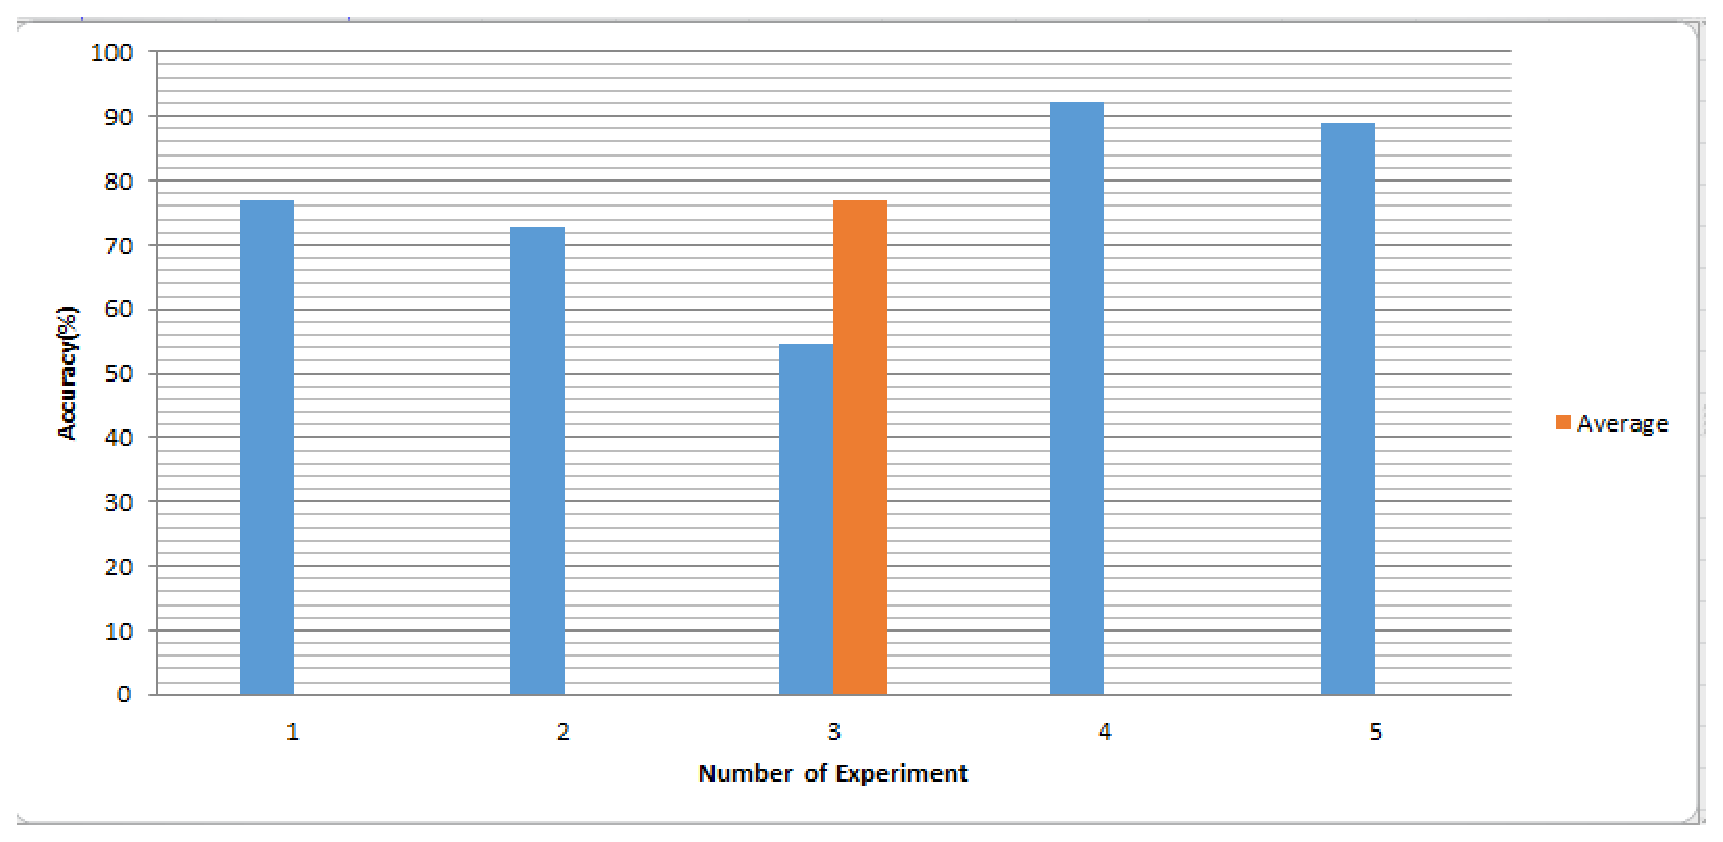
\includegraphics[width=.65\textwidth]{figure/six.eps}
	\caption{Graphical view of document ranking}
	\label{Figure:granking}
\end{figure*}


It is very difficult to determine if a ranking is good or bad. The ranking examined methods can be broadly categorized as human evaluation methods and automatic(machine-based) evaluation methods. A human evaluation is done by comparing system-generated ranking with reference model ranking by human judges.

The main problems with human evaluation are:

\begin{itemize}
	\item The evaluation process is exhausting
	\item It sustains from the lack of unity
\end{itemize}

Two human judges may not agree on each other’s judgments. Since automatic evaluation is performed by a machine, it follows a fixed logic and always produces the same result on a given ranking. Since automatic evaluation process are free from human bias, it provides a consistent way of comparing the various ranking systems.


\section{Discussion}

In this thesis, we explain the basic ideas of hoe to rank different documents according to their relevance. The ideas used are very beautiful. They are some fearsome-sounding vector space model for documents. Instead of thinking of documents and queries as strings or letters, we adopt a point of view in which both documents and queries are represented as vectors in a vector space. In this point of view, the problem of determining how relevant a document is to a query is just a question of determining how parallel the query vector and the document vector are. The more parallel the vectors, the more relevant the document is.

This geometric way of treating documents turns out to be very powerful. It’s used by most modern web search engines, including (most likely) web search engines such as Google as well as search libraries. The ideas can also be used well beyond search, for problems such as document classification, and for finding clusters of related documents.

